\documentclass[tikz,border=6pt]{standalone}
\usepackage{tikz}
\usepackage{amsmath,bm}
\usetikzlibrary{shapes.geometric, arrows.meta, positioning, fit,
                backgrounds, calc, decorations.pathreplacing}

\definecolor{threadblue}{RGB}{31,119,180}
\definecolor{regblue}{RGB}{70,130,180}
\definecolor{globalorange}{RGB}{230,136,28}
\definecolor{l2purple}{RGB}{138,43,226}
\definecolor{accentred}{RGB}{214,39,40}

\begin{document}
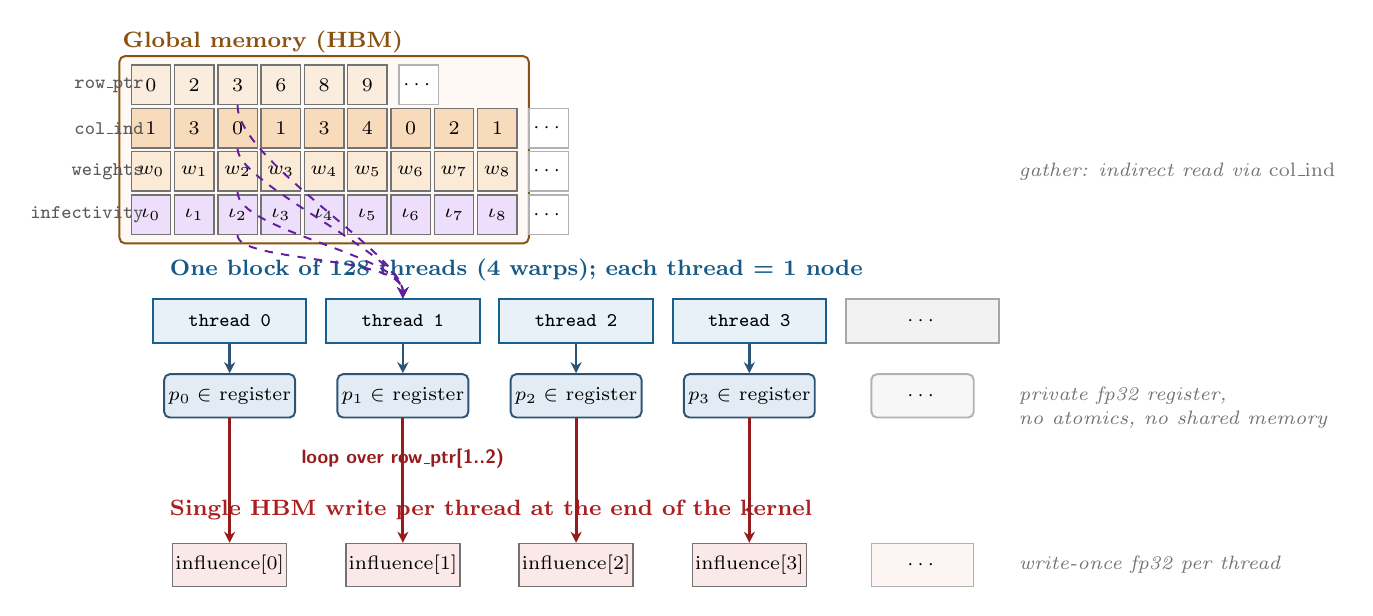
\begin{tikzpicture}[
    lane/.style={rectangle, draw=threadblue!80!black, line width=0.7pt,
                 fill=threadblue!10, minimum width=1.95cm, minimum height=0.55cm,
                 align=center, font=\scriptsize\ttfamily, inner sep=1pt},
    regbox/.style={rectangle, draw=regblue!65!black, line width=0.7pt,
                   rounded corners=2pt, fill=regblue!15,
                   minimum width=1.3cm, minimum height=0.55cm,
                   align=center, font=\scriptsize, inner sep=1.5pt},
    mem/.style={rectangle, draw=black!55, line width=0.5pt,
                fill=globalorange!15, minimum width=0.5cm, minimum height=0.5cm,
                font=\scriptsize, inner sep=1pt},
    flow/.style={-{Stealth[length=4pt,width=4pt]}, line width=0.7pt},
    gatherflow/.style={flow, color=l2purple!70!black, dashed},
    regflow/.style={flow, color=regblue!65!black, line width=0.9pt},
    writeflow/.style={flow, color=accentred!70!black, line width=1.1pt},
    lab/.style={font=\scriptsize, text=black!65, inner sep=1pt},
    annot/.style={font=\scriptsize\itshape, text=black!55},
]

%---------------------------------------------------------------
% LEFT: global CSR arrays in HBM (read source)
%---------------------------------------------------------------
\node[lab, font=\footnotesize\bfseries, text=globalorange!60!black,
      anchor=west]
     at (-0.4, 3.55) {Global memory (HBM)};

% Three rows represent the three arrays; show first few cells with "..." tail.
\foreach \v [count=\i from 0] in {0,2,3,6,8,9} {
    \node[mem] (rp\i) at (\i*0.55, 3.0) {\v};
}
\node[mem, fill=white, draw=black!30] at (6*0.55 + 0.10, 3.0) {$\cdots$};
\node[lab, anchor=east] at (-0.05, 3.0) {\texttt{row\_ptr}};

\foreach \v [count=\i from 0] in {1,3,0,1,3,4,0,2,1} {
    \node[mem, fill=globalorange!30] (ci\i) at (\i*0.55, 2.45) {\v};
}
\node[mem, fill=white, draw=black!30] at (9*0.55 + 0.10, 2.45) {$\cdots$};
\node[lab, anchor=east] at (-0.05, 2.45) {\texttt{col\_ind}};

\foreach \i in {0,1,2,3,4,5,6,7,8} {
    \node[mem, fill=globalorange!18] (ww\i) at (\i*0.55, 1.90) {$w_{\i}$};
}
\node[mem, fill=white, draw=black!30] at (9*0.55 + 0.10, 1.90) {$\cdots$};
\node[lab, anchor=east] at (-0.05, 1.90) {\texttt{weights}};

\foreach \v [count=\i from 0] in
    {$\iota_{0}$,$\iota_{1}$,$\iota_{2}$,$\iota_{3}$,$\iota_{4}$,
     $\iota_{5}$,$\iota_{6}$,$\iota_{7}$,$\iota_{8}$} {
    \node[mem, fill=l2purple!15] (inf\i) at (\i*0.55, 1.35) {\v};
}
\node[mem, fill=white, draw=black!30] at (9*0.55 + 0.10, 1.35) {$\cdots$};
\node[lab, anchor=east] at (-0.05, 1.35) {\texttt{infectivity}};

% Group label
\begin{scope}[on background layer]
    \node[fit=(rp0)(ci0)(ww0)(inf0)(inf8),
          draw=globalorange!60!black, line width=0.7pt,
          fill=globalorange!5, rounded corners=2pt,
          inner xsep=4pt, inner ysep=3pt] (hbmgroup) {};
\end{scope}

%---------------------------------------------------------------
% MIDDLE: one warp (4 lanes shown), each thread owns one node.
%---------------------------------------------------------------
\node[lab, font=\footnotesize\bfseries, text=threadblue!75!black,
      anchor=west]
     at (0.2, 0.65) {One block of 128 threads (4 warps); each thread = 1 node};

\foreach \tid [count=\k from 0] in {thread 0, thread 1, thread 2, thread 3} {
    \node[lane] (l\k) at (1.0 + \k*2.20, 0.0) {\tid};
}
\node[lane, fill=black!5, draw=black!35] at (1.0 + 4*2.20, 0.0) {$\cdots$};

% Per-thread register accumulator (float)
\foreach \k in {0,1,2,3} {
    \node[regbox] (reg\k) at (1.0 + \k*2.20, -0.95)
         {$p_{\k} \in $ register};
}
\node[regbox, fill=black!3, draw=black!30]
     at (1.0 + 4*2.20, -0.95) {$\cdots$};

% Loop indicator for thread 1 (the focus thread). Show 3 iterations of its
% CSR loop bringing in (col_ind[k], weight[k], infectivity[col_ind[k]]).
\node[lab, text=accentred!70!black, font=\scriptsize\bfseries]
     at (1.0 + 1*2.20, -1.75)
     {\textsf{loop over row\_ptr[1..2)}};

% Gather-style loads: from HBM cells to register of thread 1
\foreach \src [count=\j from 0] in {ci2, ww2, inf2, ci0} {
    % draw only a few representative arrows (to keep figure clean)
}
\draw[gatherflow] (rp2.south) .. controls ++(0, -0.7) and ++(0, 0.55) ..
     (l1.north);
\draw[gatherflow] (ci2.south) .. controls ++(0, -0.45) and ++(0, 0.55) ..
     (l1.north);
\draw[gatherflow] (inf2.south) .. controls ++(0, -0.35) and ++(0, 0.55) ..
     (l1.north);
\draw[gatherflow] (ww2.south) .. controls ++(0, -0.50) and ++(0, 0.55) ..
     (l1.north);

% Lane -> its private register accumulator.
\foreach \k in {0,1,2,3} {
    \draw[regflow] (l\k.south) -- (reg\k.north);
}

%---------------------------------------------------------------
% RIGHT: the single O(N) output written once after the loop:
% influence[i] gets a single fp32 value per thread. Also a
% pressure register drop highlighted.
%---------------------------------------------------------------
\node[lab, font=\footnotesize\bfseries, text=accentred!80!black,
      anchor=west]
     at (0.2, -2.4) {Single HBM write per thread at the end of the kernel};

\foreach \k in {0,1,2,3} {
    \node[mem, fill=accentred!10, minimum width=1.3cm,
          minimum height=0.55cm] (o\k)
         at (1.0 + \k*2.20, -3.10) {$\mathrm{influence}[\k]$};
    \draw[writeflow] (reg\k.south) -- (o\k.north);
}
\node[mem, fill=accentred!5, draw=black!30, minimum width=1.3cm,
      minimum height=0.55cm]
     at (1.0 + 4*2.20, -3.10) {$\cdots$};

%---------------------------------------------------------------
% Notes along the right margin
%---------------------------------------------------------------
\node[annot, anchor=west] at (10.9, 1.9)
     {gather: indirect read via $\mathrm{col\_ind}$};
\node[annot, anchor=west] at (10.9, -0.95)
     {private fp32 register,};
\node[annot, anchor=west] at (10.9, -1.25)
     {no atomics, no shared memory};
\node[annot, anchor=west] at (10.9, -3.10)
     {write-once fp32 per thread};

\end{tikzpicture}
\end{document}
